%\documentclass[10pt,a4paper]{article}
\documentclass[12pt,a4paper]{article}
\usepackage{graphicx,amsmath}
%\usepackage{subfigure}
\usepackage{float}
\usepackage[german]{babel}
\usepackage[utf8]{inputenc}
\setcounter{secnumdepth}{4}
\usepackage[top=2cm, bottom=2.5cm, left=3cm, right=3cm]{geometry}
\usepackage{subcaption}
\begin{document}


%\title{Bachelorarbeit}
%\author{Richard Kullmann}
%\date{02.06.2017}

\thispagestyle{empty}
%\setcounter{page}{2}
\newpage
\tableofcontents
\thispagestyle{empty}
\newpage
\pagenumbering{arabic}

\section{SNR}
Bei abnehmendem Rauschen nimmt auch das SNR ab:

\begin{figure}[H]
	\centering
	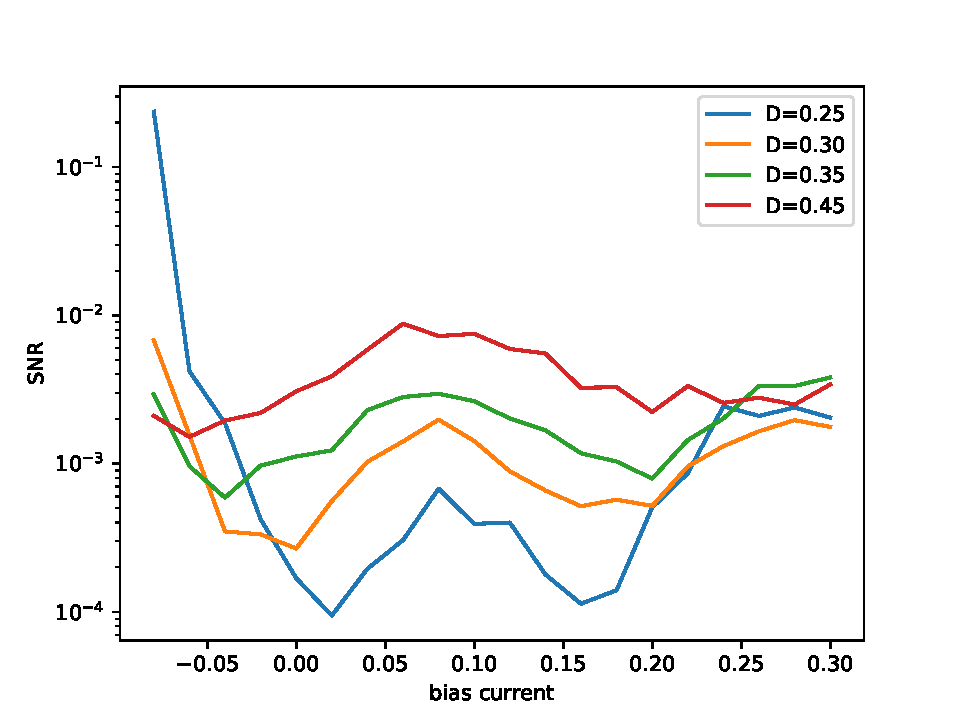
\includegraphics[scale=0.9]{snrautoreal13a25.pdf}
	\caption{SNR bei verschiedenen Rauschintensitäten}
	\label{snrnoise}
\end{figure}
Das Signal-zu-Rausch Verhältnis kann für ein Kosinus-Signal mit Stärke $\epsilon$ folgenderma"sen berechnet werden:
\begin{align*}
SNR=\frac{\epsilon ^2T}{4}\frac{|\chi(\omega)|^2}{S_0(\omega)}=\frac{\epsilon^2T|\chi(\omega)|^2}{8\cdot D_{eff}}
\end{align*}
Die Feuerraten konnten leider noch nicht vollständig numerisch ermittelt werden. Daher musste ich hier fitten:
\begin{figure}[H]
	\centering
	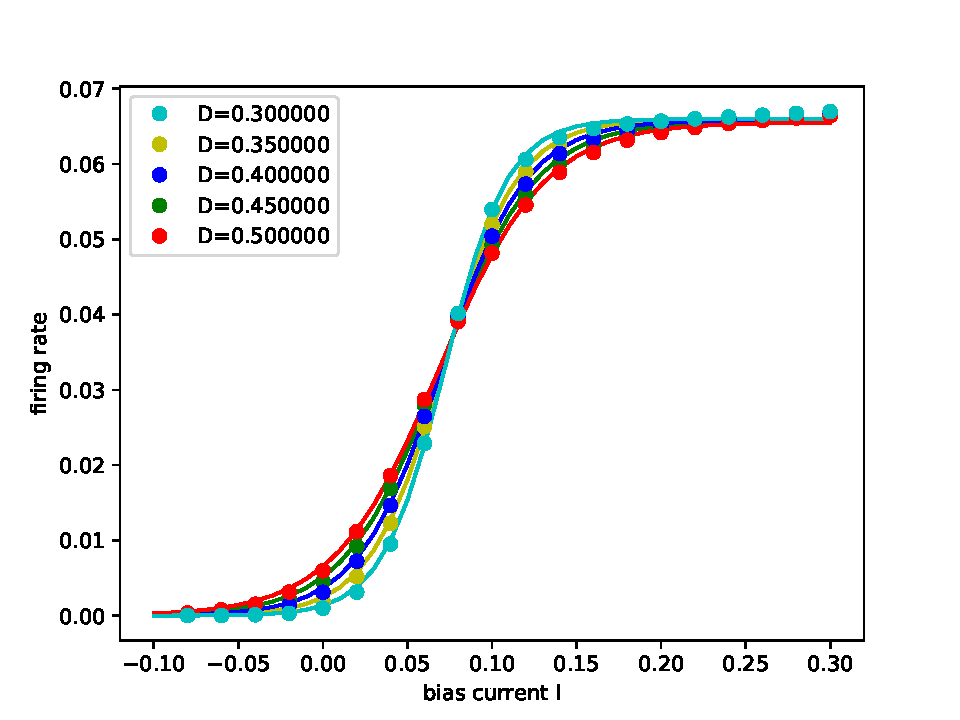
\includegraphics[scale=0.9]{gana.pdf}
	\caption{Feuerraten und entsprechende Fits}
	\label{feuerrate}
\end{figure}
Die restlichen Parameter konnten allerdings gefunden werden. Im Vergleich mit dem gemessenen SNR kann eine Übereinstimmung beobachtet werden:
\begin{figure}[H]
	\centering
	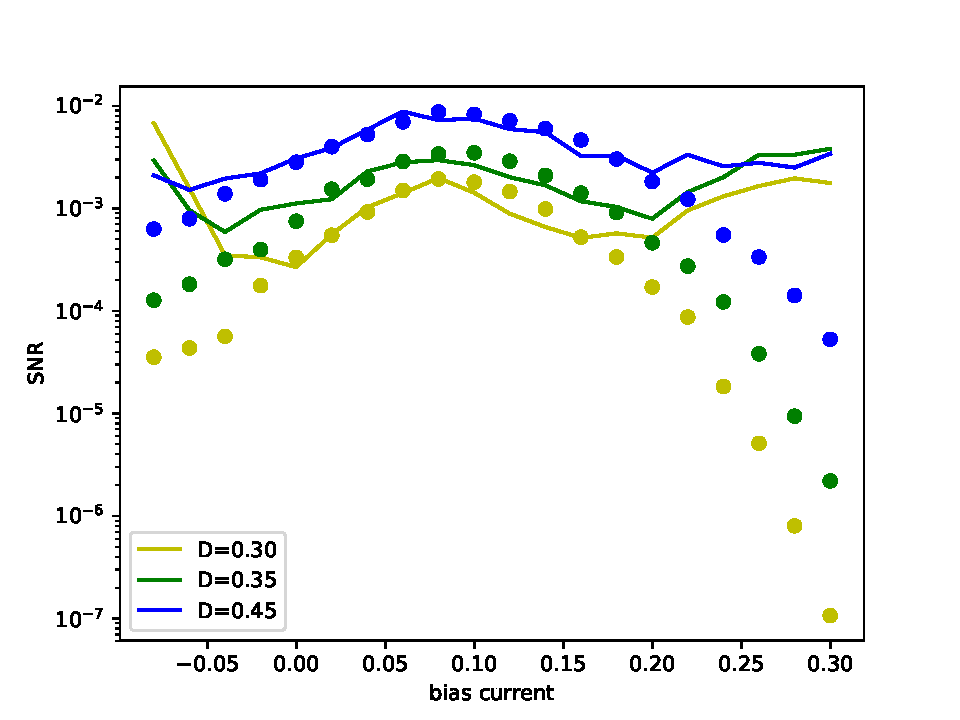
\includegraphics[scale=0.9]{snrangerealana.pdf}
	\caption{Vergleich theoretisches und gemessenes Spektrum}
	\label{deltaspectrum}
\end{figure}
Während die Maxima gut zusammenfallen, scheint das theoretische Spektrum monoton zu sein, während das gemessene Spektrum noch zwei Minima aufweist. \\
Auch das erwartete Maximum auf der SNR-Kurve in Abhängigkeit von der Rauschintensität konnte noch nicht gefunden werden:
\begin{figure}[H]
	\centering
	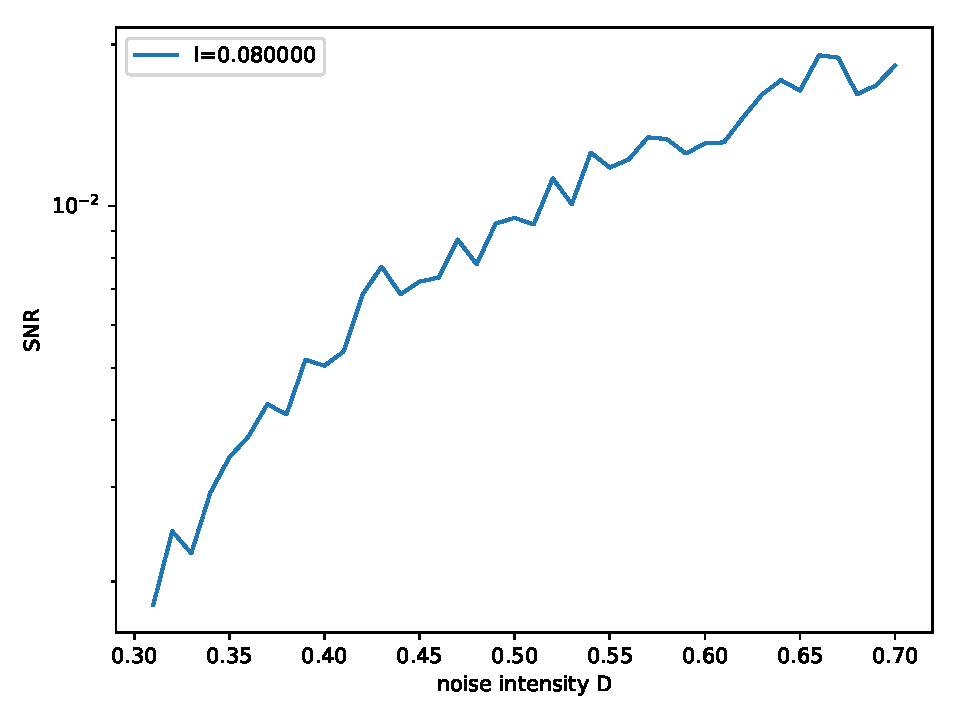
\includegraphics[scale=0.9]{snrautoabgrealdrange6aem2.pdf}
	\caption{SNR für verschiedene Werte von D}
	\label{drange}
\end{figure}
\section{Zwei-Zustands-Theorie}
Vergleicht man an jedem Punkt den gemessenen Diffusionskoeffizient mit dem Zwei-Zustands-Modell, lässt sich eine sehr gute Übereinstimmung erkennen:
\begin{figure}[H]
	\centering
	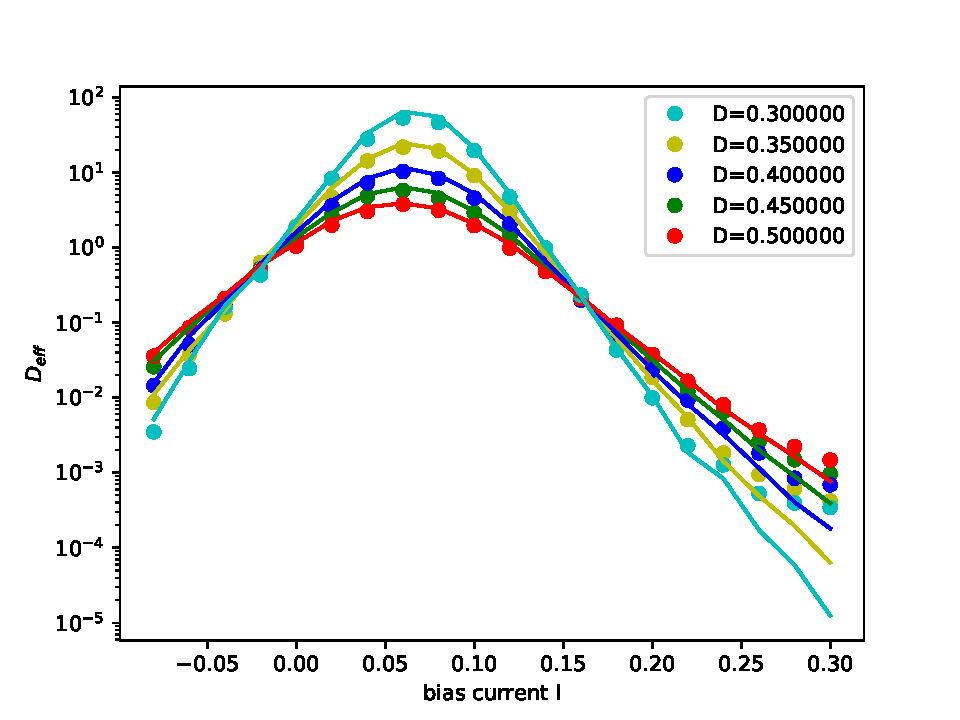
\includegraphics[scale=0.9]{dcompdfpwnewrealfast11jjem2shrealfast19jjem2st.pdf}
	\caption{Vergleich Diffusionskoeffizient und Zwei-Zustands-Theorie}
	\label{dcomp}
\end{figure}
Das quadratische Fitten der Potentialbarrieren liefert ein deutlich besseres Ergebnis als der lineare Ansatz:
\begin{figure}[H]
	\centering
	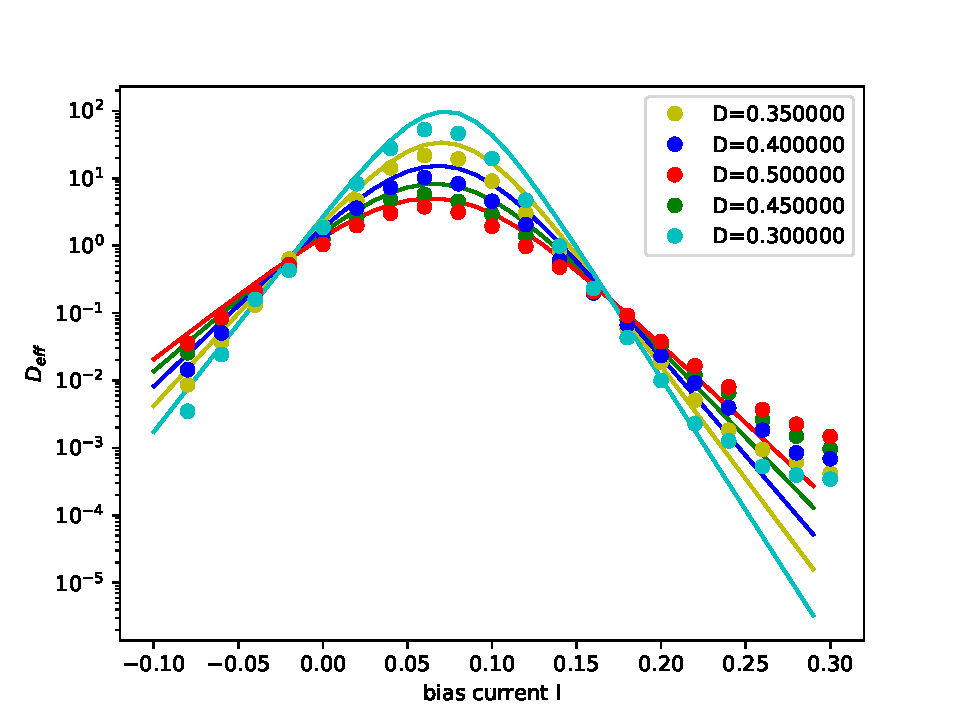
\includegraphics[scale=0.9]{dcompdfnewrealfast11jjem2shrealfast19jjem2st.pdf}
	\caption{Vergleich Diffusionskoeffizient und verallgemeinerter Zwei-Zustands-Theorie mit linearen Barrieren}
	\label{dcomplin}
\end{figure}
\begin{figure}[H]
	\centering
	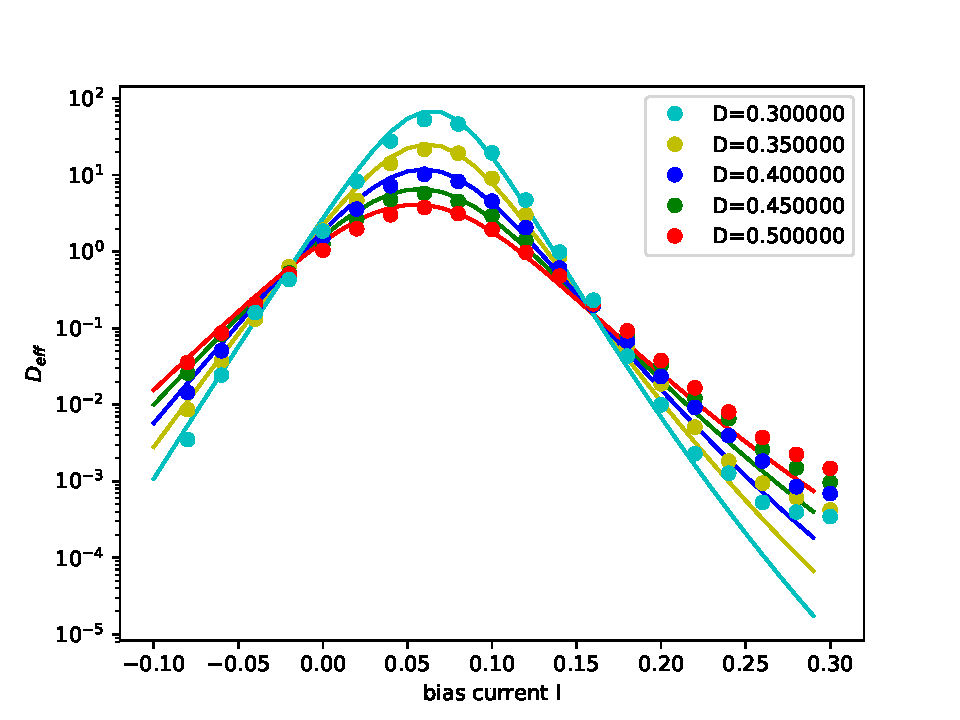
\includegraphics[scale=0.9]{dcompdfqnewrealfast11jjem2shrealfast19jjem2st.pdf}
	\caption{Vergleich Diffusionskoeffizient und verallgemeinerte Zwei-Zustands-Theorie mit quadratischen Barrieren}
	\label{dcompqua}
\end{figure}
Daher ist es auch nicht überraschend, dass das SNR mit dem allgemeinen Zwei-Zustands-Modell gut angenähert wird:
\begin{figure}[H]
	\centering
	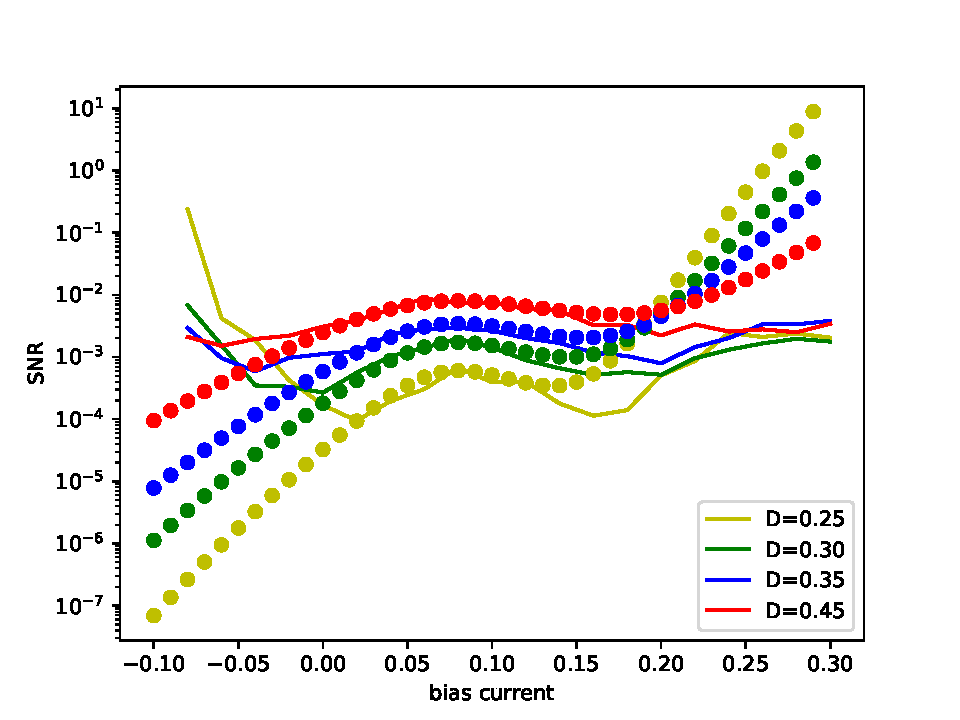
\includegraphics[scale=0.9]{snrautoreal13a25snr.pdf}
	\caption{Vergleich SNR mit der verallgemeinerten Zwei-Zustands-Theorie mit quadratischen Barrieren}
	\label{snrtwo}
\end{figure}
\section{Einfluss der Parameter}
\begin{figure}[H]
	\centering
	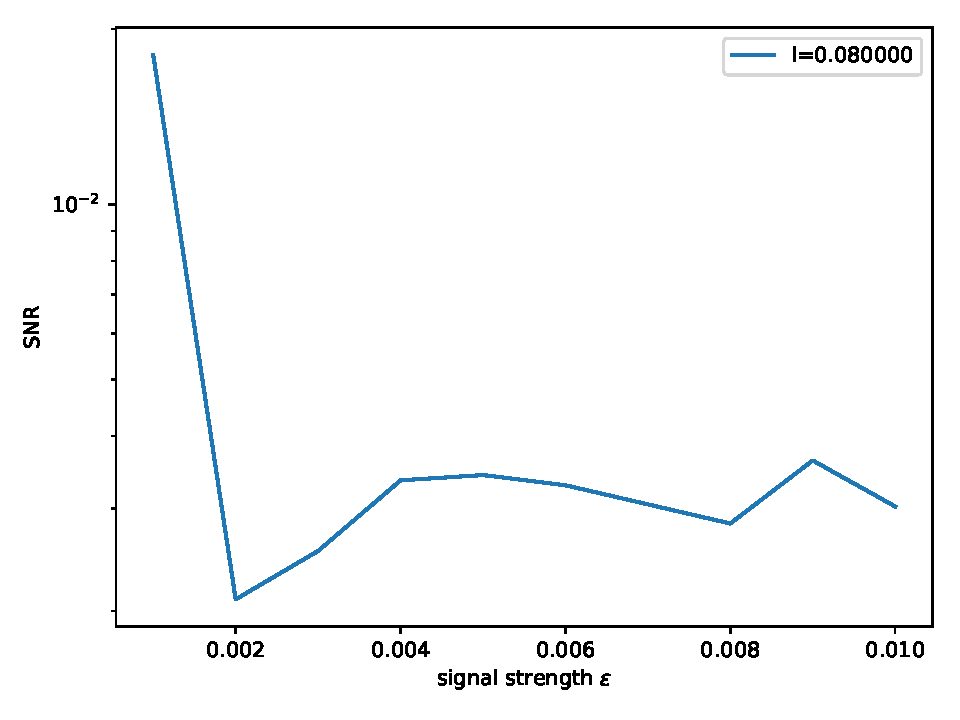
\includegraphics[scale=0.9]{snrepsautorealdrange6aem2.pdf}
	\caption{Abhängigkeit des gemessenen SNR von der Signalstärke}
	\label{eps}
\end{figure}
\end{document}